\section{Introduction}

Au $XXI^e$ siècle, les batteries sont devenues un des axes majeurs de développement en chimie. L'apparition ces dernières décennies d'un nombre croissant de technologies autonomes comme les smartphones, les véhicules électriques, certains équipements médicaux (pompe à insuline, stimulateur cardiaque$\ldots$) ont fait naître le besoin de développement de systèmes de stockage miniaturisés. Aujourd'hui, comme nous l'expliquerons par la suite, c'est l'élément chimique lithium et ses technologies dérivées qui offrent les meilleures perspectives en terme d'ergonomie (miniaturisation, poids$\ldots$), d'efficacité énergétique et de coût de production.

\begin{minipage}[c]{0.65\textwidth}
\centering
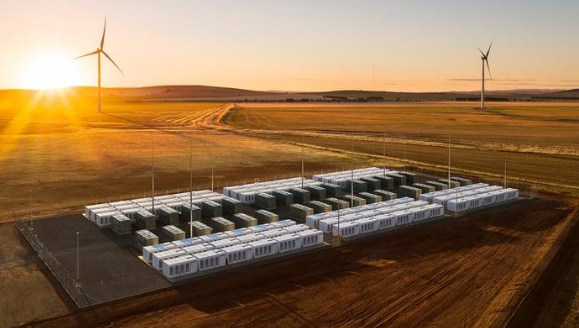
\includegraphics[width=5cm]{figures-Chp0/3-Reseau.png}
\end{minipage}\hfill   
\begin{minipage}[c]{0.35\textwidth}     
\captionof{figure}{Installation d'un centre de stockage d'énergie éolienne, par Tesla, en Autralie exploité par le groupe français Neoen [tiré de la \href{https://www.maisondelenergie.fr/sites/maisondelenergie.fr/files/batteries_1.pdf}{maison de l'énergie, batteries}]}
\label{tab:battery_reseau}
\end{minipage}

Bien entendu, à l'heure de la transition écologique, accompagnée du développement des énergies renouvelables, l'intégration des systèmes de stockage de masse au sein des réseaux électriques constitue un enjeu. En effet, les énergies renouvelables : photovoltaïque, éolien, nucléaire sont des sources d'énergies moins flexibles que le charbon ou le gaz. Les deux premières présentent une dépendance aux conditions environnementales quand la dernière présente une production constante. Au sein du réseau électrique, l'intégration de batteries, en général sodium-soufre, permet une meilleure maîtrise des pics ou déficits de tension électrique.

Dans notre cas, l'étude des batteries sera décomposée en trois temps. Dans un premier temps, des rappels des notions d'électricité et d'électrochimie seront faites que vous soyez capable d'appréhender l'analyse des batteries. Dans un second temps, vous vous intéresserez aux méthodes analytiques permettant de mesurer l'efficacité d'une batterie. Dans un dernier temps, vous caractérisez une batterie lithium et vérifierez son adéquation à un cahier des charges.

\objectif{
La liste ci-dessous décrit les compétences à acquérir durant ce TP.

~

\faBattery[0] Notions élémentaires : 
\begin{itemize}
    \item pile vs accumulateur \& batterie primaire vs secondaire ;
    \item oxydant vs réducteur \& oxydation vs réduction ;
    \item composante d'une cellule : électrodes, électrolyte, séparateur ;
    \item anode vs cathode \& conventions générateur/récepteur ;
    \item potentiels rédox, interpréter la spontaneité ou non d'une réaction électrochimique ;
    \item courant, tension, puissance électrique, rendement en charge et en énergie d'une cellule.
\end{itemize}

\faBattery[2] Comprendre comment caractériser l'efficacité d'une batterie.
\begin{itemize}
    \item Mesure de l'état d'une pile : SoC, DoD et SoH ;
    \item Utiliser et interpréter une courbe tension-temps dans le cadre d'un cycle de charge et décharge ;
    \item Utiliser les rendements de charge et de décharge afin de caractériser la charge et la décharge.
\end{itemize}

\faBattery[4] Savoir diagnostiquer les propriétés électrochimiques d'une batterie.
\begin{itemize}
    \item Comprendre que les performances d'une batterie ou accumulateur peuvent être caractérisées par la capacité électrique, la puissance délivrable et la cyclabilité de la pile ;
    \item Caractériser l'état de charge et de décharge d'une batterie : SoC \& DoD ;
    \item Caractériser l'état de santé d'une pile : SoH ;
    \item Identifier les sources d'hystérèses entre la charge et la décharge ;
    \item Comprendre et poser des hypothèses sur les sources de vieillissement d'une batterie.
\end{itemize}}

\newpage

\chapter{\faBattery[0] Notions élémentaires à usage dans les batteries}

Une batterie est un dispositif qui stocke de l'énergie sous forme chimique et qui le restitue sous forme d'énergie électrique. Lors de ce processus, deux espèces chimiques rédox, c'est-à-dire des espèces chimiques capables d'échanger un ou plusieurs électrons, réagissent ensemble. Cette réaction libère de l'énergie sous deux formes : 
\begin{itemize}
    \item un travail utile \textbf{W'} qui est le travail électrique ;
    \item une déperdition d'énergie, la chaleur \textbf{Q}, c'est-à-dire de l'énergie thermique.
\end{itemize}

\begin{minipage}[c]{0.65\textwidth}
\centering
\includegraphics[width=5cm]{figures-Chp0/4-FirstPrinciple.png}
\end{minipage}\hfill   
\begin{minipage}[c]{0.35\textwidth}     
\captionof{figure}{Représentation des flux reçus par une batterie.}
\label{tab:battery_W_Q}
\end{minipage}

La batterie est parfois à usage unique ou rechargeable. Ainsi, si la batterie est rechargeable, le travail électrique est soit reçu $W' > 0$ (charge) ou cédé $W' < 0$ (décharge). En son sein, des éléments résistifs imposent que la batterie perd nécessairement, que ça soit en charge ou décharge, une partie de son énergie sous forme thermique $Q < 0$.

Cette capacité à recevoir ou non du travail électrique permet de classifier les batteries en plusieurs catégories.

\section{Classification des générateurs électrochimiques}

\begin{figure}[H]
\begin{centering}
\subfloat[\label{fig:cir_gen}]{\includegraphics[height=3cm]{figures-Chp0/5-CircuitGen}}\subfloat[\label{fig:cir_gen_sch}]{\includegraphics[height=3cm]{figures-Chp0/5-CircuitGen-Sch}}\hfill\subfloat[\label{fig:cir_rec}]{\includegraphics[height=3cm]{figures-Chp0/5-CircuitRec}}\subfloat[\label{fig:cir_rec_sch}]{\includegraphics[height=3cm]{figures-Chp0/5-CircuitRec-Sch}}
\par\end{centering}
{\tiny{}\caption{{\small{} Fig. \ref{fig:cir_gen}) Représentation schématique d'une pile AAA alimentant d'une résistance et une diode électroluminescente rouge ; Fig. \ref{fig:cir_gen_sch}) Circuit électrique équivalent ; ig. \ref{fig:cir_rec}) Représentation schématique d'une pile AAA et d'une résistance alimentée par un générateur en mode DC ; Fig. \ref{fig:cir_rec_sch}) Circuit électrique équivalent.}}
}{\tiny\par}
\end{figure}%WARNING : mettre U_B pour la tension de la batterie

Les générateurs électrochimiques peuvent être classifiés en deux grandes catégories : 

\subsection{Dispositifs constitués d'une seule cellule électrochimique}

\paragraph*{La pile électrique} est un dispositif électrochimique qui génère de l'électricité en convertissant de l'énergie chimique en énergie électrique grâce à une réaction d'oxydoréduction. 

Du point de vue électrique, la pile est donc un \textbf{générateur électrique} dont la réaction d'oxydoréduction est \textbf{irréversible}. Seul le cas, illustré Fig. \ref{fig:cir_gen}/\ref{fig:cir_gen_sch} est possible.

\paragraph*{L'accumulateur} est un dispositif électrochimique qui génère (resp. reçoit) de l'électricité en convertissant de l'énergie chimique (resp. électrique) en énergie électrique (resp. chimique) grâce à une réaction d'oxydoréduction réversible. 

Du point de vue électrique, l'accumulateur est :
\begin{itemize}
\item un \textbf{générateur électrique} lorsqu'il se décharge ;
\item un \textbf{récepteur électrique} lorsqu'il se charge
\end{itemize}
dont la réaction d'oxydoréduction est \textbf{réversible}. Les deux cas, illustré Fig. \ref{fig:cir_gen}/\ref{fig:cir_gen_sch} \& \ref{fig:cir_rec}/\ref{fig:cir_rec_sch} sont possibles.

\subsection{Dispositifs constitués de plusieurs cellules électrochimiques}

\paragraph*{La batterie} est le nom donné à tout dispositif électrique résultant de la mise en série et/ou en parallèle de plusieurs piles ou accumulateurs. On les classe alors en deux catégories : 
\begin{enumerate}
    \item Primaire lorsque l'on a mis en série des piles ;
    \item Secondaire lorsqu'on l'on a mis en série des accumulateurs.
\end{enumerate}

Ainsi, tout générateur primaire ne peut être utilisé qu'une unique fois, et doit être jeté après utilisation. 

\section{Réactions électrochimiques}
Avant d'aborder la structure d'une batterie, il est important de remettre en place quelques termes de vocabulaire propre aux réactions électrochimiques.

\paragraph*{Oxydant/Réducteur}

Dans ce type de réaction, l'une des espèces cède des électrons, c'est le réducteur et l'autre en gagne, c'est l'oxydant. 
\begin{center}
    \begin{align*}
        \underbrace{\ce{Cu^{2+}}}_{oxydant} (aq) + \underbrace{\ce{Zn(s)}}_{réducteur} &= \ce{Cu (s)} + \ce{Zn^{2+} (aq)}
    \end{align*}
\end{center}

\exercice{
\Q \label{Q:1.1} Dans chacune des réactions suivantes, indiquer l'oxydant et le réducteur :
\begin{enumerate}
    \item \ce{Li (s) + H2O (l) = Li^+ (aq) + HO^- (aq) + \frac{1}{2} H2 (g)} ;
    \item \ce{PbO2 (s) + Pb (s) + 2 H2SO4 (aq) = 2PbSO4 (aq) + 2 H2O (l)}
\end{enumerate}}


\paragraph*{Oxydation/Réduction}

Afin de modéliser le flux d'électron, il est possible de décomposer l'équation de réaction en deux demi-équations rédox modélisant chacune une oxydation (le couple qui libère des électrons) et une réduction (le couple qui gagne des électrons).
\begin{center}
\begin{minipage}{0.4\textwidth}
\begin{align*}
    \ce{Cu^{2+} (aq) + 2e^- &= Cu (s)}\\
    \ce{Zn(s) &= Zn^{2+} (aq) + 2e^- } \\
    \hline
    \ce{Cu^{2+}(aq)  + Zn(s) &= Cu (s) + Zn^{2+} (aq)} 
\end{align*}
\end{minipage}    
\end{center}

\exercice{\Q En reprenant les équations de réaction \ref{Q:1.1}, indiquer la demi-équation rédox et si il s'agit de la modélisation d'une oxydation/réduction sachant que les couples rédox mis en jeux sont les suivants :
\begin{enumerate}
    \item \ce{Li^+ (aq)} / \ce{Li (s)} \& \ce{H2O (l)}/\ce{H2 (g)} ; 
    \item \ce{PbO2} (s) / \ce{Pb^{2+} (aq)} \& \ce{Pb^{2+}} (aq) / \ce{Pb (s)}%voir peut-être retirer SO42-
\end{enumerate}}


\subsection{Description d'une batterie}
La description que nous allons faire traite de manière indifférente les batteries primaires et secondaires. En ces termes, piles et accumulateurs porteront le nom générique de cellule.

Toute cellule est un dispositif composé de $\ldots$

\paragraph*{$\ldots$ deux électrodes} dont l'une sert à capter les électrons et l'autre sert à céder des électrons. Une cellule est, par conséquent, un \textbf{dipôle électrique orienté}.

%WARNING : image pour orienter le dispositif électrique.

Chaque électrode joue un rôle précis, et son nom vous informe sur le processus physico-chimique mis en jeu : 
\begin{minipage}[c]{0.65\textwidth}
\centering
\begin{tabular}{ccc}
\toprule
\textbf{Type d'électrode} & \textbf{anode} & \textbf{cathode}  \\
\midrule
Réaction électrochimique & oxydation & réduction \\
Générateur & $\ominus$ & $\oplus$ \\
Récepteur & $\oplus$ & $\ominus$ \\
\bottomrule
\end{tabular}
\end{minipage}\hfill   
\begin{minipage}[c]{0.35\textwidth}     
\captionof{figure}{Conventions de nom et d'orientation électrique d'un accumulateur.}
\label{tab:conventions}
\end{minipage}




Dans le cas d'une pile Daniell, pile galvanique aqueuse utilisant les couples \ce{Cu^{2+}(aq)}/\ce{Cu(s)} et \ce{Zn^{2+}(aq)}/\ce{Zn(s)}, le dispositif peut se présenter de la manière suivante :

\begin{minipage}[c]{0.65\textwidth}
\centering
\includegraphics[width=8cm]{figures-Chp0/6-Diode-Voltmeter.png}
\end{minipage}\hfill   
\begin{minipage}[c]{0.35\textwidth}     
\captionof{figure}{Pile Daniell réalisée à l'aide :}
\begin{itemize}
    \item d'une solution de sulfate de cuivre accompagné d'une plaque de cuivre (cathode) ;
    \item d'une solution de sulfate de zinc accompagné d'une plaque de zinc (anode) ;
\end{itemize}

L'ensemble est fermé d'une part par un pont salin contenant une solution de \ce{KNO3} concentrée et d'autre part par un circuit électrique fermé.
\label{fig:pileCuZn_Exp}
\end{minipage}


Schématiquement, le dispositif s'écrit comme : 
\begin{equation}
\oplus \quad \ce{Cu(s)} | \ce{Cu^{2+} (aq)}; \ce{SO_4^{2-} (aq)} | K^+ (aq), NO_3^- (aq) | \ce{Zn^{2+} {aq}}; \ce{SO_4^{2-} (aq)} | \ce{Zn(s)} \quad \ominus
\label{eq:pileCuZn}
\end{equation}

où les $|$ indiquent les interfaces entre les différentes phases.


%WARNING : retrouvver l'infos
\paragraph*{$\ldots$ solvant} Le solvant est l'espèce permettant solvatant les espèces électroactives et électrolytiques.

Dans la pile Daniell, le solvant est l'eau.

\paragraph*{$\ldots$ séparateur} En général, les cellules sont composées d'un séparateur qui est une membrane ou un pont qui permet de séparer \textbf{physiquement} et \textbf{spécifiquement} les espèces électroactives du compartiment anodique et cathodique. Ce séparateur obéit à deux contraintes : empêcher toute réaction parasite entre espèces électroactives, tout en assurant une bonne conductivité ionique d'espèces chimiques chargées, mais inertes chimiquement.

Dans la pile Daniell, le pont salin est le séparateur.

\paragraph*{$\ldots$ électrolyte} Afin de fermer le circuit électrique, au sein de la pile, le courant doit être conduit. Contrairement aux fils et électrodes, où le courant est assuré par les électrons, dans la solution et le séparateur, le courant est assuré par la \textbf{migration} des ions. C'est ce qu'on appelle l'\textbf{électrolyte}.

Celui-ci obéit à deux contraintes : 
\begin{enumerate}
    \item diminuer la résistivité des compartiments anodiques et cathodiques ;
    \item garantir le processus de migration au sein de la solution.
\end{enumerate}

En effet, la résistance à la conduction ionique est souvent l'une des principales sources de déperdition de l'énergie chimique en chaleur. C'est ce que, tout bon électrochimiste que vous êtes, appellera \textbf{la chute ohmique} (c'est-à-dire la déperdition d'énergie sous forme d'énergie thermique à cause de la loi d'Ohm). Le second point ne sera abordé qu'en cours d'électrochimie avec Alireza Ranjbari.

{\Large \faWarning } Parfois, l'électrolyte support peut-être une ou plusieurs espèces électroactives. Dans la pil Daniell présentée Fig. \ref{fig:pileCuZn_Exp}, c'est le cas.

\exercice{
Les batteries utilisées couramment dans les véhicules électriques, mais également dans d'autres applications comme les téléphones portables, sont de type lithium-ion. Elles présentent l'avantage d'avoir une très grande énergie massique, comprise entre 90 et \SI{180}{\watt\hour\per\kilo\gram}. De plus, ces batteries, même partiellement déchargées, délivrent toujours la même puissance, ce qui permet une utilisation dans les mêmes conditions, quel que soit le niveau de charge. Le principe général d'une batterie lithium-ion est basé sur l'échange réversible des ions lithium entre une électrode positive en oxyde métallique (\ce{MO2}) et une électrode négative en graphite qui va stocker les ions lithium pendant la charge :

~

\begin{minipage}[c]{0.65\textwidth}
\centering
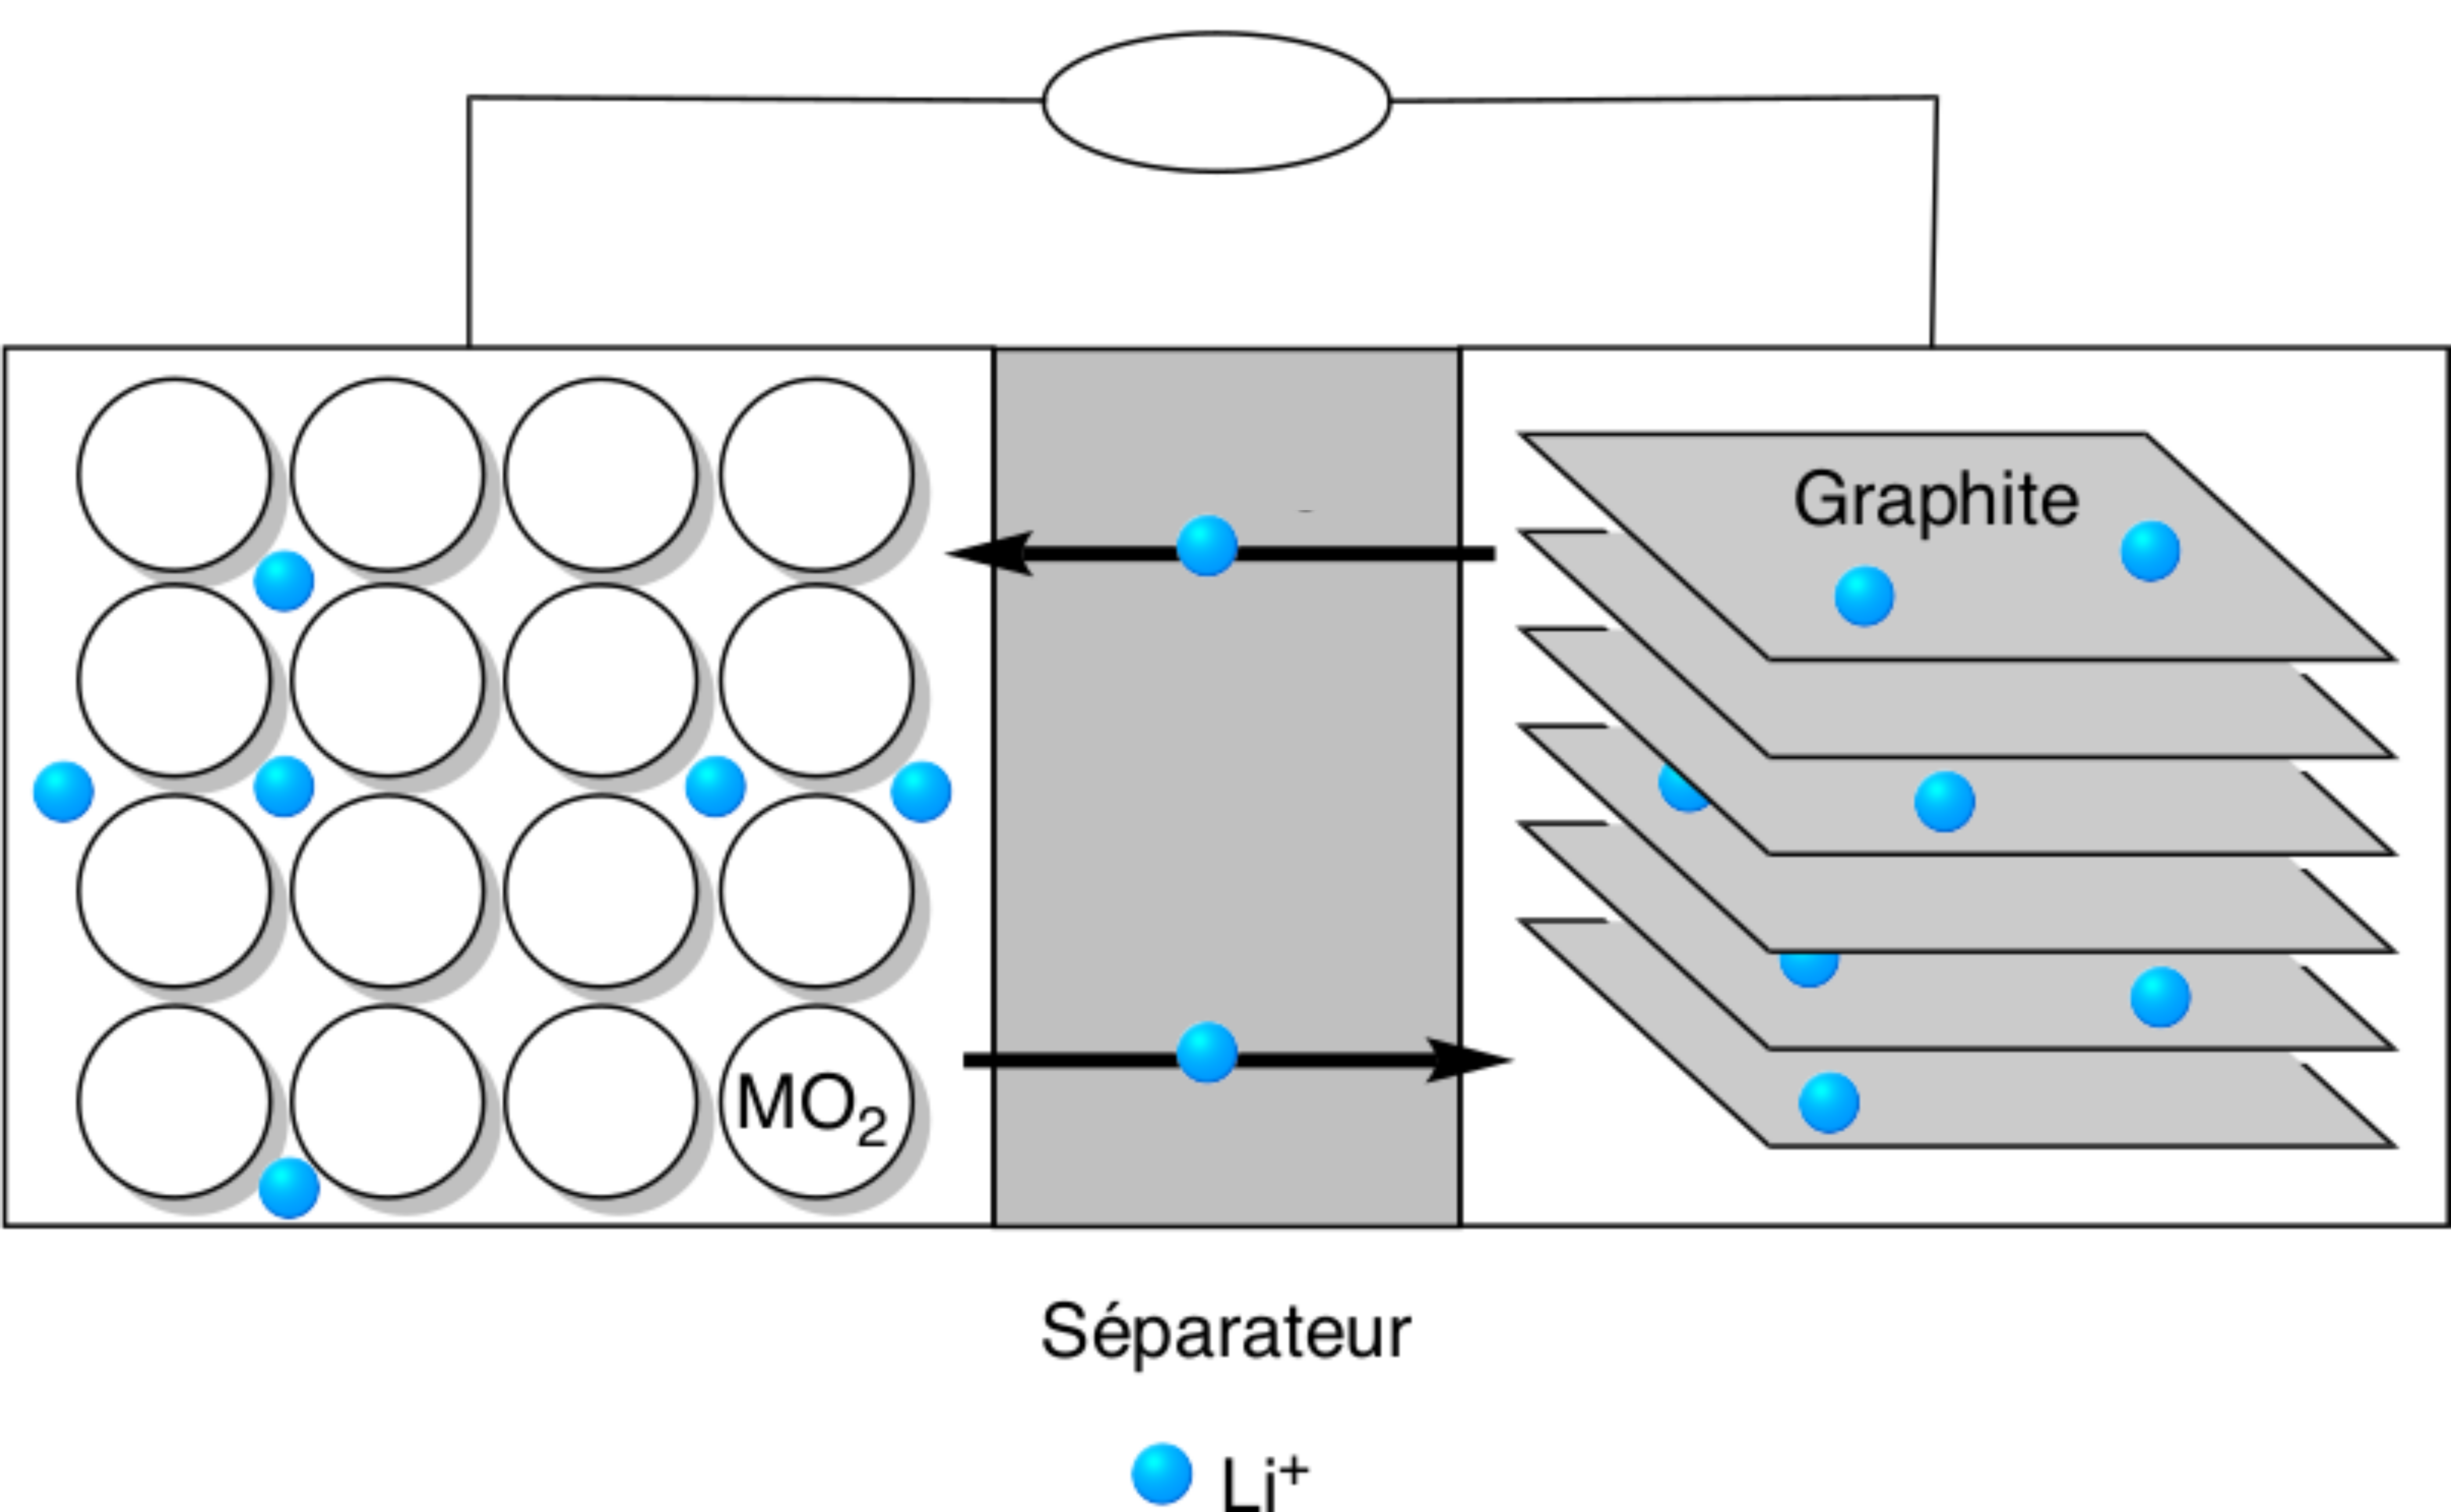
\includegraphics[width=6cm]{figures-Chp0/7-BatteryLithium.png}
\end{minipage}\hfill   
\begin{minipage}[c]{0.35\textwidth}     
\captionof{figure}{Technologie au lithium-ion. Le solvant utilisé est une espèce organique.}
\label{fig:li-ion}
\end{minipage}

\Q En vous appuyant sur la représentation du graphite, expliqué pourquoi les ions Li peuvent s'insérer entre les feuillets de graphite. On sait que le rayon ionique du lithium est de \SI{60}{\pico\meter} et le covalent est de \SI{134}{\pico\meter}.

\begin{minipage}[c]{0.65\textwidth}
\centering
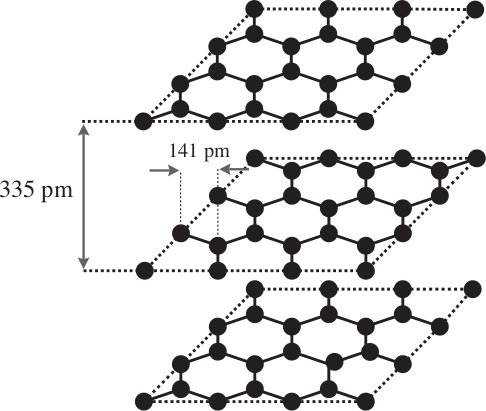
\includegraphics[height=4cm]{figures-Chp0/11-graphene.png}
\end{minipage}\hfill   
\begin{minipage}[c]{0.35\textwidth}     
\centering
\captionof{figure}{Structure du graphite}
\label{fig:graphite}
\end{minipage}

\Q A l'état totalement chargé, la structure du composé est \ce{LiC6}. Écrire la demi-équation rédox à cette électrode lors de la charge et de la décharge et préciser le signe de l'électrode de graphite.
La seconde électrode peut être en oxyde de cobalt (\ce{CoO2}) qui, après insertion des ions lithium,
forme l'oxyde lithié \ce{LiCoO2}. 
\Q Montrer que c'est l'élément cobalt qui change de degré d'oxydation ;
\Q Donner la demi-équation électronique associée au couple considéré lors de la charge et de la décharge
à cette électrode en précisant son signe.
\Q Reproduire et orienter le schéma de la Fig. \ref{fig:li-ion} dans le cas d'une charge puis d'une décharge. Vous indiquerez le nom et le signe des électrodes puis le flux d'électron, le courant électrique et la direction de migration des ions lithium.
%tiré de Mines-Pont 2022.

~

La suite de cet exercice sera traité à la partie suivante.}

\section{Caractériser un accumulateur ou une batterie}

\subsection{Charge, \'{E}nergie \& Puissance}
Les cellules électrochimiques sont des dispositifs électriques. Par conséquent, trois grandeurs électriques usuelles permettent de les caractériser : la charge (notée \textbf{C}), la tension (notée \textbf{U}) et le courant (notée \textbf{I}). Le courant dérive de la charge.

Deux grandeurs dérivées des trois grandeurs fondamentales de l'électricité peuvent nous intéresser :

\begin{enumerate}
    \item la puissance électrique instantannée, notée $P$
    \begin{equation}
        P(t) = U(t) I(t)
        \label{eq:puissance}
    \end{equation}
    \item le travail électrique, noté $W'$
    \begin{equation}
        W' = \int_0^t P(t') dt' = \int_0^t U(t') I(t') dt'
        \label{eq:travail}
    \end{equation}
\end{enumerate}

Lorsque le dispositif électrique est en convention récépteur (resp. générateur), la relation Eq.\ref{eq:puissance} nous donne la puissance \textbf{reçue} (resp. émie) par le dispositif. De même pour la relation sur le travail Eq.\ref{eq:travail}.

Bien entendu, toutes ces grandeurs sont à mettre en perspective avec la durée de vie d'un accumulateur. Tant qu'il présente une tension et une énergie stockée stable malgré les cycles de charge et de décharge, on peut considérer qu'il est fonctionnelle. Cette notion est appelée \textbf{cyclabilité}, c'est-à-dire le nombre de cycles de charge/décharge pendant lesquelles ces paramètres restent constants.

\exercice{
\Q Donner le signe de la puissance et du travail lorsqu'une cellule électrochimique est un récepteur reçoit de l'énergie. Même chose si il s'agit d'un générateur.

Dans les batteries, la puissance électrique est un critère de second plan. Ce qui intéresse principalement les industriels s'est que l'énergie délivrée par la batterie puisse stocker une grande quantité d'énergie, tout en la débitant de manière pérenne dans le temps.

\begin{center}
\begin{adjustbox}{width=0.95\textwidth}
\begin{tabular}{cccccc}
    \toprule
     \textbf{Technologie} & \textbf{Année de développement} & \textbf{Energie massique} & \textbf{Energie volumique} & \textbf{Tension} & \textbf{Cyclabilité}\\
     Unité & & \si{\watt\hour\per\kilo\gram} & \si{\watt\hour\per\liter} & \si{\volt}/au couple \ce{Li^+}/\ce{Li} & $\emptyset$ \\
     \midrule
     Plomb & 1859 & 35 & 70 & 2.0 & 200-250\\
     Nickel-Cadmium & 1900 & 60 & 100 & 1.2 & 400-500\\
     Nickel-Métal-Hydrure & 1975 & 80 & 240 & 1.2 & 400-500\\
     Lithium-Ion & 1978 & 250 & 400 & 3.6 & > 1000\\
     \bottomrule
\end{tabular}   
\end{adjustbox}
\captionof{table}{\small \'{E}volution des ordres de grandeurs de l'énergie massique, volumique, de la tension ainsi que de la cyclabilité d'une batterie en fonction de la technologie.}
\label{tab:battery_time}
\end{center}


\Q Commenter les valeurs de la Tab.\ref{tab:battery_time}. Quel est l'intérêt de la technologie Li-ion par rapport à d'autres technologies ?
\Q Mettre en relation ces données avec la place de l'élément Li au sein du tableau périodique.}



\subsection{État de charge et état de santé}
Afin de caractériser l'état d'une pile ou batterie, on peut utiliser diverses grandeurs caractéristiques permettant de définir son état à un instant $t$.

\paragraph*{\'{E}tat de charge (SoC, State-of-Charge)} L'état de charge d'une batterie indique la quantité d'énergie emmagasinée par la batterie. On la définit comme : 
\begin{equation*}
    SoC [\si{\percent}]= \frac{\text{charge emmaganisé par la batterie}}{\text{charge maximale que peut emmaganiser la batterie}} * 100
    \label{eq:SoC}
\end{equation*}

Si $SoC =$ \SI{0}{\percent} (resp. \SI{100}{\percent}), la batterie est déchargée (resp. chargée)


\paragraph*{\'{E}tat de décharge (DoD, Depth-of-Discharged)} L'état de décharge d'une batterie indique la quantité d'énergie non emmagasinée par la batterie. On la définit comme : 
\begin{equation*}
    DoD [\si{\percent}]= \frac{\text{charge non emmaganisé par la batterie}}{\text{charge maximale que peut emmaganiser la batterie}} * 100
    \label{eq:DoD}
\end{equation*}

Par définition, $DoD [\si{\percent}] = 100 - SoC [\si{\percent}]$. Si $DoD =$ \SI{0}{\percent} (resp. \SI{100}{\percent}), la batterie est chargée (resp. déchargée)

\paragraph*{\'{E}tat de santé (SoH, State-of-Health)} L'état de santé d'une batterie indique la charge maximale réelle par rapport à la charge maximale théorique que peut contenir la batterie.
\begin{equation*}
    SoH [\si{\percent}]= \frac{\text{charge maximale réelle}}{\text{charge maximale théorique}} * 100
    \label{eq:SoH}
\end{equation*}

L'état de santé permet de caractériser l'état de vieillissement de votre pile. Si la pile est neuve (resp. usagée), alors $SoH =$ \SI{100}{\percent} (resp. $SoH \to$ \SI{0}{\percent}).

\exercice{%sujet central 2022

Suite de l'exercice$\ldots$

\Q Déterminer l'expression de la capacité de la batterie (en \si{\ampere\hour\per\kilo\gram}) en fonction du nombre d'électrons échangés, de la constante de Faraday et de la masse molaire du matériau d'insertion (le graphite).

Pour le véhicule considéré, équipé d'une batterie lithium-ion dont les caractéristiques sont fournies dans le \textbf{Document}, la jauge d'autonomie de la batterie indique \SI{20}{\percent}. Son conducteur souhaite la recharger et pour cela, il utilise une borne de recharge qui fournit une puissance constante de \SI{7.40}{\kilo\watt} en délivrant un courant électrique d'intensité constante de \SI{32.0}{\ampere}.

\Q Calculer l'énergie massique maximale de la batterie considérée (\textbf{Document}). Commenter.

\Q Calculer l'énergie emmagasinée par la batterie lors de sa charge pour passer d'un SOC de \SI{20}{\percent}
à \SI{80}{\percent} et définir le rendement de la charge, puis le calculer. Commenter cette valeur.

Récemment, des chercheurs, en utilisant une anode composée de feuillets de graphène et de \ce{SnO2} sont parvenus à réaliser une batterie dont la capacité spécifique est de \SI{635}{\milli\ampere\hour\per\gram} après 100 cycles charge/décharge, la capacité spécifique étant à l'origine de \SI{784}{\milli\ampere\hour\per\gram}. La diminution de la capacité spécifique est liée à la grande surface spécifique du graphène et est due à la perte irréversible d'ions lithium, du fait de la décomposition de l'électrolyte, qui précipite et passive la surface de l'anode accessible pour la lithiation.

\Q Calculer l'état de santé de cette batterie.

\Q Estimer la perte de surface spécifique pour la batterie étudiée par les chercheurs.

~

\textbf{Document}

~

\emph{La technologie lithium-ion est communément utilisée dans les batteries des voitures électriques. Les principales caractéristiques d'une batterie Li-ion présente dans le véhicule électrique considéré dans
cette étude sont les suivantes :}

~

\begin{minipage}[c]{0.65\textwidth}
\centering
\begin{tabular}{cc}
     \'{E}nergie utilisable & \SI{41}{\kilo\watt\hour} \\
     Tension totale & \SI{400}{\volt} \\
     Nombre de cellules & 192 \\
     Masse de la batterie & \SI{305}{\kilo\gram} \\
\end{tabular}
\end{minipage}\hfill   
\begin{minipage}[c]{0.35\textwidth}     
    \captionof{table}{Principale caractéristique d'une batterie Li-ion d'un véhicule électrique.}
    \label{tab:li-ion_car}
\end{minipage}

~

\emph{Pour la batterie considérée, la variation SoC en fonction du temps de charge de la batterie est donnée à la figure suivante : }

~

\begin{minipage}[c]{0.65\textwidth}
\centering
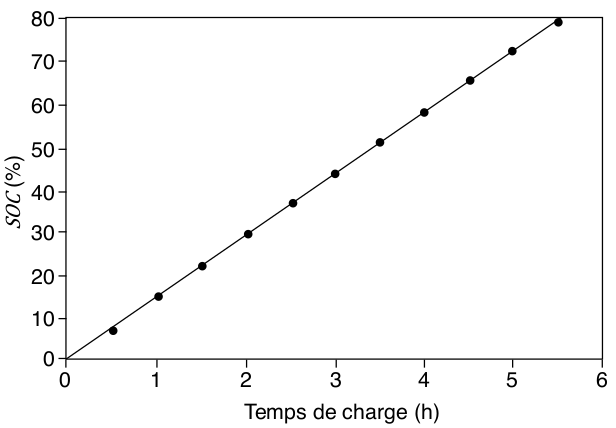
\includegraphics[width=6cm]{figures-Chp0/10-SoC.png}
\end{minipage}\hfill   
\begin{minipage}[c]{0.35\textwidth}     
    \captionof{figure}{\'{E}volution du SoC en fonction du temps de charge.}
    \label{fig:li-ion_car}
\end{minipage}
}